
% This is LLNCS.DEM the demonstration file of
% the LaTeX macro package from Springer-Verlag
% for Lecture Notes in Computer Science,
% version 2.2 for LaTeX2e
%
\documentclass{llncs}
%%%%%%%%%%%%%%%%%%%%%%%%%%%%
% *** MISC UTILITY PACKAGES ***
%
\usepackage{ifpdf}

% *** CITATION PACKAGES ***
\usepackage{cite}

% *** GRAPHICS RELATED PACKAGES ***
%
\usepackage[pdftex]{graphicx}

% *** MATH PACKAGES ***
\usepackage[cmex10]{amsmath}

% *** SPECIALIZED LIST PACKAGES ***
\usepackage{algorithmic}

%SP: Added to reduce verticle space between the subsections
\setlength{\topskip}{0pt}

% *** ALIGNMENT PACKAGES ***
\usepackage{array}
\usepackage{mdwmath}
\usepackage{mdwtab}
%\usepackage{eqparbox}

% *** SUBFIGURE PACKAGES ***
%\usepackage[tight,footnotesize]{subfigure}
\usepackage{caption}
\usepackage{subcaption}

% *** FLOAT PACKAGES ***
\usepackage{fixltx2e}

%\usepackage{stfloats}
% stfloats.sty was written by Sigitas Tolusis. This package gives LaTeX2e
% the ability to do double column floats at the bottom of the page as well
% as the top. (e.g., "\begin{figure*}[!b]" is not normally possible in
% LaTeX2e). It also provides a command:
%\fnbelowfloat
% to enable the placement of footnotes below bottom floats 

% *** PDF, URL AND HYPERLINK PACKAGES ***
\usepackage{url}

% correct bad hyphenation here
\hyphenation{Shar-ed Memo-ry Pass-ing  Mess-age Be-sides bench-mark su-pports uni-versity Carolina}

\usepackage{flushend}
\usepackage{listings}
\usepackage{color}
\usepackage{framed}  %package for framing images
\usepackage{lscape}
\usepackage{hyperref}
%\usepackage{subfig}
\usepackage{float}
\usepackage{multirow}

%\usepackage[options]{algorithm}

%\floatstyle{boxed} 
\restylefloat{figure}

\setcounter{secnumdepth}{5}
% NOTE:
%\section{} % level 1
%\subsection{}  %level 2
%\subsubsection{} % level 3
%\paragraph{} % level 4 - equivalent to subsubsubsection
%\subparagraph{} % level 5
% 
\definecolor{dkgreen}{rgb}{0,0.6,0}
\definecolor{gray}{rgb}{0.5,0.5,0.5}
\definecolor{mauve}{rgb}{0.58,0,0.82}
 
\lstset{ 
  language=C,                     % the language of the code
  %basicstyle=\footnotesize, 
  basicstyle=\ttfamily\scriptsize,      % the size of the fonts that are used for the code
  numbers=left,                   % where to put the line-numbers
  numberstyle=\tiny\color{gray},  % the style that is used for the line-numbers
  stepnumber=1,                   % the step between two line-numbers. If it's 1, each line 
                                    % will be numbered 
  backgroundcolor=\color{white},  % choose the background color. You must add \usepackage{color}
  showspaces=false,               % show spaces adding particular underscores
  showstringspaces=false,         % underline spaces within strings
  showtabs=false,                 % show tabs within strings adding particular underscores
  rulecolor=\color{black},        % if not set, the frame-color may be changed on line-breaks within not-black text (e.g. commens (green here))
  tabsize=1,                      % sets default tabsize to 2 spaces
  %captionpos=b,                   % sets the caption-position to bottom
  breaklines=true,                % sets automatic line breaking
  breakatwhitespace=true,        % sets if automatic breaks should only happen at whitespace
  %title=\lstname,                 % show the filename of files included with \lstinputlisting;
  caption=\lstname,                                 % also try caption instead of title
  keywordstyle=\color{blue},          % keyword style
  commentstyle=\color{dkgreen},       % comment style
  stringstyle=\color{mauve},         % string literal style
  escapeinside={\%*}{*)},            % if you want to add LaTeX within your code
  xleftmargin=15pt,
  morekeywords={*,...}              % if you want to add more keywords to the set
}
%%%%%%%%%%%%%%%%%%%%%%%%%%%%
\usepackage{makeidx}  % allows for indexgeneration
%
\lstset{numbers=left,numberblanklines=false,escapeinside=||}
\let\origthelstnumber\thelstnumber
\makeatletter
\newcommand*\Suppressnumber{%
  \lst@AddToHook{OnNewLine}{%
    \let\thelstnumber\relax%
     \advance\c@lstnumber-\@ne\relax%
    }%
}

\newcommand*\Reactivatenumber{%
  \lst@AddToHook{OnNewLine}{%
   \let\thelstnumber\origthelstnumber%
   \advance\c@lstnumber\@ne\relax}%
}
%%%%%%%%%%%%%%%%%%%%%%%%%%%%%%%%%%%%%%%%%%%%%%%%%%%%%%%%%%%%%
\begin{document}
%
\frontmatter          % for the preliminaries
%
\pagestyle{headings}  % switches on printing of running heads
%\mainmatter              % start of the contributions
%%
\title{Evaluating OpenMP Affinity on the POWER8 Architecture }

%Affinity evaluation in OpenMP 4.5  
%Affinity and accelerators - using device_num, data regions for the accelerator, however none of these mechanism are aware of NUMA domains.
%Using the OpenMP 4.5 target data directive it could be a mechanism to control affinity
%
%Places in the OpenMP 4.5 we need a new way to specify a NUMA domain in the context of a device. 
%
%#pragma omp target data device(host:NUMA1) map(tofrom: a, b: zerocopy)  
%{
%
%#pragma omp target device(host:NUMA1) 
%pragma omp parallel 
% // these threads belong to the NUMA node.  
%  // NUMA domain
%
%}



%
%\titlerunning{Hamiltonian Mechanics}  % abbreviated title (for running head)
%                                     also used for the TOC unless
%                                     \toctitle is used
%
\author{Swaroop Pophale \and Oscar Hernandez
}
%
%%%% modified list of authors for the TOC (add the affiliations)
\tocauthor{Swaroop Pophale, Oscar Hernandez (Oak Ridge National Laboratory)}
%
\institute{
Computer Science and Mathematics Division\\
Oak Ridge National Laboratory, Oak Ridge, Tennessee, 37840, USA\\
\email{\{pophaless,oscar\}@ornl.gov}
}
\maketitle              % typeset the title of the contribution

\begin{abstract}
As we move toward pre-Exascale systems, two of the DOE leadership class systems will consist of very powerful OpenPOWER compute nodes which which will be more complex to program. These will have massive amounts of parallelisms where threads may be running on Power9 cores as well as on accelerators. Advances in memory interconnects, such as NVLINK, will provide a unified shared memory address spaces for different types of memories HBM, DRAM, etc.

In preparation for such system, we need to improve our understanding on how OpenMP supports the concept of affinity as well as memory placement on current state-of-
the art systems, and if this work needs to be extended to support heterogenous systems that will have massive amounts of threads. Data locality and affinity are key 
concepts to exploit the compute and memory capabilities to achieve good performance by minimizing data motion across NUMA domains. This  paper is the first step to 
evaluate the current features of OpenMP 4.0 on the Power8 processors, and on how to measure its effects on a system with two P8 sockets. We experiment with the 
different affinity settings provided by OpenMP 4.0 affinity to quantify the costs of having good data locality vs not,  and measure their effects via hardware counters. We also 
find out which affinity settings benefits more from data locality. Based on this study we describe the current state of art, the challenges we faced in quantifying effects of 
affinity, and and ideas on how OpenMP 5.0 should be improved to address affinity in the context of accelerators and NUMA domains.


% Importance of affinity, it is well understood for traditional systems but lil understanding on massively multi-threaded heterogeneous architectures (including the different memories). OpenMP implicitly controls affinity but there is no explicit way to control memory hierarchy.
\end{abstract}

\section{Introduction}
% How affinity works on 4.0 and 4.5
% What discussions are being proposed for 5.0 --telecon
\label{sec:intro}
The effects of affinity is a widely studied problem. Most programming models 
take advantage of the architecture and data-access patterns by providing some 
implicit or explicit control over data and process/thread placement. For example,
Partitioned Global Address Space (PGAS) languages/APIs provide mechanisms to specify 
globally accessible data (with local views) and memory affinities to physical memory. 
For example, UPC provides a \textbf{shared} qualifier to distinguish between data 
accessible to all the UPC \textit{threads} vs. private data and distribution keywords to place
the data on different affine memories. For arrays UPC provides 
three affinity granularities: blocked, cyclic and blocked-cyclic. 
%The \textit{shared} scalar data has 
%affinity to thread 0, while arrays can have affinity granularity of \textit{cyclic, blocked-cyclic ,}
%and \textit{blocked}. These are chosen by the application programmer based on the 
%knowledge of the data access patterns within the application. 

OpenMP being a shared memory programming models, it has 
different ways to specify and affect affinity of data, threads, and work units or \textit{tasks}. 
The new OpenMP 4.0 release provides a substantial 
improvement on the support for programming of accelerator and GPU devices. 
Amongst the new features introduced are, support for parallelization of loops with 
well-structured dependencies, mechanisms for unstructured data mapping and 
asynchronous execution, support to divide loops into tasks without requiring all 
threads to execute the loop, reductions for C/C++ arrays, a new hint mechanisms to 
provide guidance on the relative priority of tasks and on preferred synchronization 
implementations, SIMD extensions, improved support for Fortran 2003, and
thread affinity support through runtime functions to determine the effect of thread 
affinity clauses. In this paper we focus on the affinity aspect of OpenMP with respect 
to the emerging OpenPOWER systems.

\subsection{Memory Binding}
Most systems provide implicit data affinity control through policies like \textit{first-touch} 
and \textit{next-touch}. First-touch is more appropriate for applications where the 
first access to data is representative of the application\'s data accesses throughout 
the life of the application. This policy has been adopted as default on many systems. 
For applications that have a more dynamic access pattern, the \textit{next-touch} 
policy may be more appropriate. Here the data is marked to be placed on the node of the 
next CPU that accesses it. For OpenMP, \textit{first-touch} translates to data being 
placed near the thread that first accesses it. Even without any other affinity mechanism this 
can cause significant impact, for e.g., if the data is initialized by thread 0 only, but later is accessed 
by all the threads, the \textit{first-touch} policy would locate memory on the node where 
thread 0 is placed thus resulting in high cost accesses for threads not placed on the same node. 

\subsection{Thread Placement}
OpenMP provides OMP\_PROC\_BIND ICV to set the thread affinity policy. The legitimate value for 
this environment variable is either true, false, or a comma separated list of master, close, or spread. 
When the values are specified in a list, they correspond to the thread affinity policy to be used for 
parallel regions at the corresponding nested level. In combination with the OMP\_PLACES ICV, 
users may have complete control on the thread affinity and their placement on a given hardware. 
OMP\_PLACES ICV can be one of two types of values: either an abstract name describing a set 
of places or an explicit list of places described by non-negative numbers. Pre-defined abstract 
names include \textit{threads, cores,} and \textit{sockets}. When expressed as numbers, places 
represent the smallest unit of execution exposed by the execution environment, which is typically 
a hardware thread.

In conjunction to places represented by non-negative numbers, intervals is another handy way to 
express \textit{places} in OpenMP. They are specified using the \textit{$<$lower-bound$>$ : $<$length$>$ : $<$stride$>$} notation. For example, a user could specify exact CPUs to place the OpenMP threads or a range of CPUs based on the application characteristics to best utilize the underlying hardware.
\subsection{POWER8 System}
%Needs to be paraphrased 
The POWER8 processor is the latest RISC (Reduced Instruction Set Computer) microprocessor from IBM and the first processor supporting the new OpenPOWER software environment. 
%End paraphrase
The IBM POWER8 system has three possible configurations of either 6, 10 or 12 (6 X 2) cores per processor chip. A typical 12 core processor, as shown in Figure~\ref{fig:p8_1} has  512 KB SRAM L2 caches per core, 96 MB eDRAM shared L3 and an off chip L4 cache that provides up to 128 MB eDRAM space. 
\begin{figure}
    \centering
    \begin{subfigure}[b]{0.4\textwidth}
         {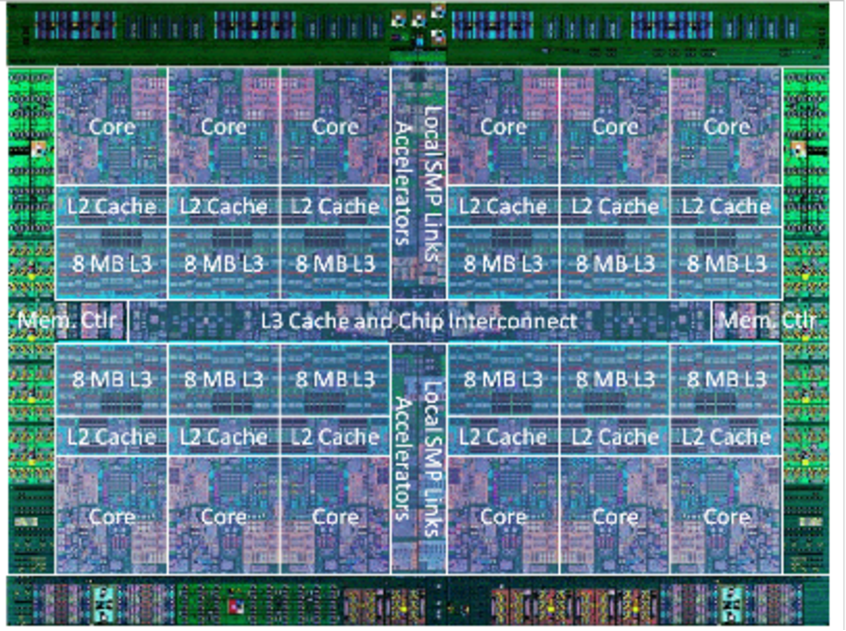
\includegraphics[width=1.0\textwidth]{./Images/P8.pdf}}
%  	\vspace{-0.0pc}
	 \caption{Power8 processor chip.~\cite{IBM_P8}}
 	 \label{fig:p8_1}
    \end{subfigure}
     \centering
    \begin{subfigure}[b]{0.4\textwidth}
         {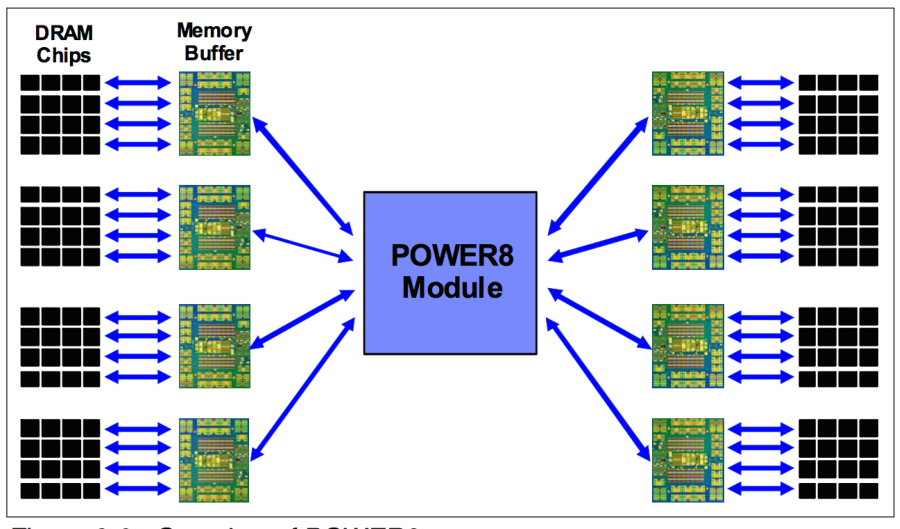
\includegraphics[height=0.7\textwidth]{./Images/P8_memory.pdf}}
  %	\vspace{-0.0pc}
	 \caption{Power8 Memory Access.~\cite{IBM_P8}}
	  \label{fig:p8_2}
    \end{subfigure}
  \caption{POWER8 Overview}\label{fig:POWER8}
\end{figure}
The POWER8 system has a Non-Uniform Cache Architecture (NUCA) Cache Policy, this allows for scalable bandwidth and latency, allowing migration of most used cache lines to the local L2 cache and then to the local L3 cache~\cite{IBM_P8}. This is a big improvement over the POWER7 processor.  Each cache level will have a cost for accessing data locally vs remote.  

%When we run the command  \textit{numactl} the operating system reports the following NUMA nodes on a two socket POWER8 system. 
A NUMA distance is the ratio between the latency of accessing  a remote numa node memory and local memory access. To illustrate this,  when we run the command \textit{numactl} on a two socket POWER8 system, we get the following 
NUMA nodes and distances (see ~\ref{fig:crest}): 

\begin{figure}[h]
  \centering
  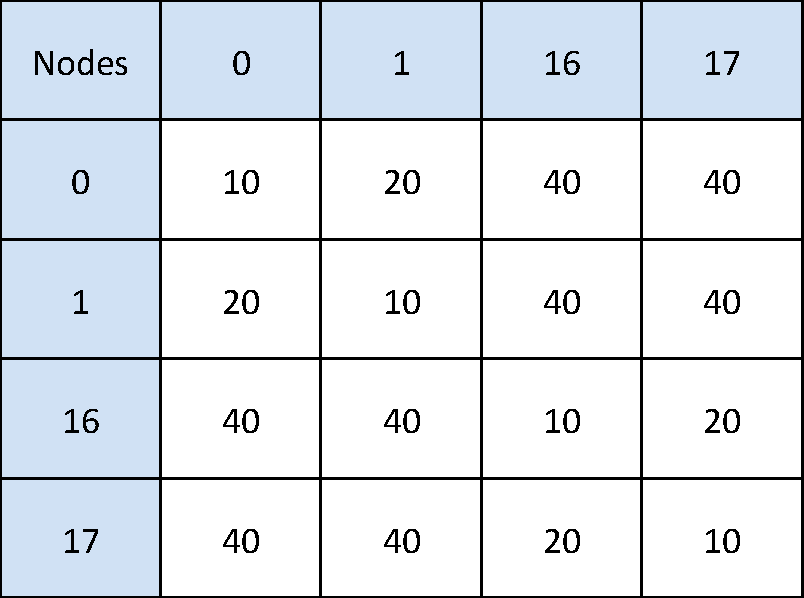
\includegraphics[height=0.3\textwidth]{./Images/crest.pdf}
       \caption{\textit{Numactl} hardware characteristics of a two socket POWER8 system}
       \label{fig:crest}
\end{figure}

%[4/9/16, 12:37:55 PM] Oscar: we just need to expand the text for that table
%[4/9/16, 12:38:07 PM] Oscar: we need to explain why we have these numbers in blue
%[4/9/16, 12:38:25 PM] Oscar: and why we have these many rows and columns
%[4/9/16, 12:38:38 PM] Oscar: and how that related to a dual socket POWER8 system



 

%\section{Motivation}
%How do affinity constructs work and see their adequacy and propose extensions ---on OpenPOWER 
%\label{sec:motivation}
%The new Exascale system at ORNL, Summit, will be an OpenPOWER system with NVIDIA GPUs. To provide a better understand of the working of OpenMP 
programs on this novel architecture we look at the most impactful aspects of the programming model. By examining the POWER8 hardware counters while testing the OpenMP 4.0 affinity features implemented in different compilers available on the new system, we hope to measure effects of affinity at scale. Based on this study, we describe the challenges that we faced in quantifying effects of affinity, inadequacy in the current OpenMP programming model and how some of these may be addressed in OpenMP 5.0. We also endeavor to find the optimum OpenMP settings for different application kernels that can yield the best performance.

\section{Motivation}
\label{sec:method}
To understand the relationship between OpenMP affinity and data locality in the POWER8 architecture we want to quantify the effect of data locality under different combinations of OMP\_PROC\_BIND and OMP\_PLACES settings and quantify their effects using the available POWER8 hardware counter information.

\subsection{POWER8 Hardware Counters}
To quantify the effects of data affinity and data locality, we look closely at the different hardware counters available on the POWER8 memory subsystem, including \textbf{data cache} stall cycles. Long cache latencies and cache misses usually indicate poor placement of data with respect to the executing thread in a OpenMP program. Performance instrumentation in POWER8 is provided in two layers: the \textbf{Core Level Performance Monitoring} (CLPM) and the \textbf{Nest Level Performance Monitoring} (NLPM). CLPM allows for monitoring of the core pipeline efficiency of the front-end, branch prediction, schedulers etc., along with behavioral metrics such as stalls, execution rates, thread prioritization and resource sharing, and utilizations of resources etc. On the other hand NLPM provides a way to instrument the L3 cache, interconnect fabric and memory channels/controllers. 
%
\begin{table*}[h]
\vspace{-0.5pc}
\centering
\begin{tabular} { | l | l |}
\hline
%PM\_CMPLU\_STALL\_
*DCACHE\_MISS & Stall by Data Cache (L1) misses\\  \hline
%PM\_CMPLU\_STALL\_
*DMISS\_L2L3 & Stall by Dcache miss which resolved in L2/L3 \\  \hline
%PM\_CMPLU\_STALL\_
*DMISS\_L2L3\_CONFLICT & Stall due to cache miss due to L2 L3 conflict \\  \hline
%PM\_CMPLU\_STALL\_
*DMISS\_L2L3\_NO\_CONFLICT & Stall due to cache miss due to L2 L3 conflict \\ \hline
%PM\_CMPLU\_STALL\_
*DMISS\_L3MISS & Stall due to cache miss resolving missed the L3 \\ \hline
%PM\_CMPLU\_STALL\_
*DMISS\_LMEM & GCT empty by branch mispredict + IC miss\\ \hline
%PM\_CMPLU\_STALL\_
*DMISS\_L21\_L31 &  Stall by Dcache miss which resolved on chip \\ \hline%(excluding local L2/L3)\\ \hline
%PM\_CMPLU\_STALL\_
*DMISS\_REMOTE  & Stall by Dcache miss which resolved from remote chip \\ \hline%(cache or memory)\\ \hline
%PM\_CMPLU\_STALL\_
*DMISS\_DISTANT & Stall by L1 reloads from distant interventions and memory \\ \hline
 \end{tabular}
 \caption{Explanation of the Data Cache Miss Stall Counters on POWER8 \\ * = PM\_CMPLU\_STALL\_}
\label{tab:hwct}
\end{table*}
%
POWER8 has an enhanced Cycles Per Instruction (CPI) Accounting Model. The POWER8 CPI Stack accounts for stalled, waiting to complete, thread blocked, completion table empty, completion and other miscellaneous cycles. The stalled cycles are further classified based on the cause of the stall. Newly added to this group for the POWER8 architecture is the finer granularity of \textit{Stall cycles due to Dcache Misses}.  Since we want to quantify cycles wasted due to data misses due to NUCA and NUMA latencies, we focus on the sub-set of hardware counters mentioned in Table~\ref{tab:hwct}. The collection of the counter values are enabled by a system provided script. This allows for access to counters that may not be represented as literary strings and accessible via other application profiling tools. PM\_CMPLU\_STALL\_DCACHE\_MISS is a combination of stall cycles 
%
\begin{table*}[h]
%\vspace{-0.5pc}
\centering
\begin{tabular} { | l | l |}
\hline
 \multirow{2}{*} {PM\_CMPLU\_STALL\_DMISS\_L2L3} & PM\_CMPLU\_STALL\_DMISS\_L2L3\_CONFLICT  \\ 
   & PM\_CMPLU\_STALL\_DMISS\_L2L3\_NO\_CONFLICT  \\ \hline
   \multirow{4}{*} {PM\_CMPLU\_STALL\_DMISS\_L3MISS} &	PM\_CMPLU\_STALL\_DMISS\_LMEM \\ 
   & PM\_CMPLU\_STALL\_DMISS\_L21\_L31  \\ 
   & PM\_CMPLU\_STALL\_DMISS\_REMOTE  \\ 
   & PM\_CMPLU\_STALL\_DMISS\_DISTANT \\ \hline
 \end{tabular}
 \caption{Relationship between different Data Cache Miss Stall Counters on POWER8}
\label{tab:cl}
\end{table*}
%
\subsection{Experimental Setup}
\subsubsection{Test System}
We use the experiment POWER8 system at the Oak Ridge National Laboratory for our experiments. This system consists of two POWER8 sockets with four chiplets that map to NUMA nodes. Ten CPUs arranged over two sockets have the capacity to support 8 threads per CPU, thus providing a total of up to 160 threads for computation. The system has 256GB of main memory memory.
% four NVIDIA Tesla K40m GPUs, two Mellanox Connect-IB InfiniBand FDR (56 Gb/s) ports and one 4-port Gigabit Ethernet switch. 

\subsubsection{The Experiment}
To able to identify the correlation between hardware counters and OpenMP affinity features we use the Jacobi iterative method program to solve a 
finite difference discretization of Helmholtz equation (here on referred to as \textit{Jacobi program}). We vary the affinity of data by controlling the initialization loop at the start of the program. 
When affinity characteristic is \textit{true}, all threads initialize the data arrays in parallel using the omp\_parallel construct, this allows for the 
\textit{first-touch} policy described in Section~\ref{sec:intro} to place data closer to the physical CPU executing the OpenMP thread. When 
affinity characteristic is \textit{false}, only the master thread (thread 0) will initialize the data causing data to be placed only around the physical CPU executing thread 0. We then test combinations of OpenMP \textit{bindings} and \textit{places} and collect the performance data and the values of the hardware counters mentioned in Table~\ref{tab:hwct}.

Based on this information we hope to see a co-relation between the POWER8 hardware counters and data-affinity of the executing program. 
%The ultimate aim of this experiment is to be able to \textit{suggest} the correct combination of OpenMP \textit{bindings} and \textit{places} based on 
%either the range, ratio or value of the different hardware counters. %methodology, implementation and results here

\section{Results}
\label{sec:results}
As explained in Section~\ref{sec:intro} OpenMP 4.0 provides two environment variables OMP\_PROC\_BIND and OMP\_PLACES to help users define the thread placement for their shared memory OpenMP application which together we refer to as \textit{OpenMP Affinity}.%
%\begin{figure}[h!]
%  \centering
%  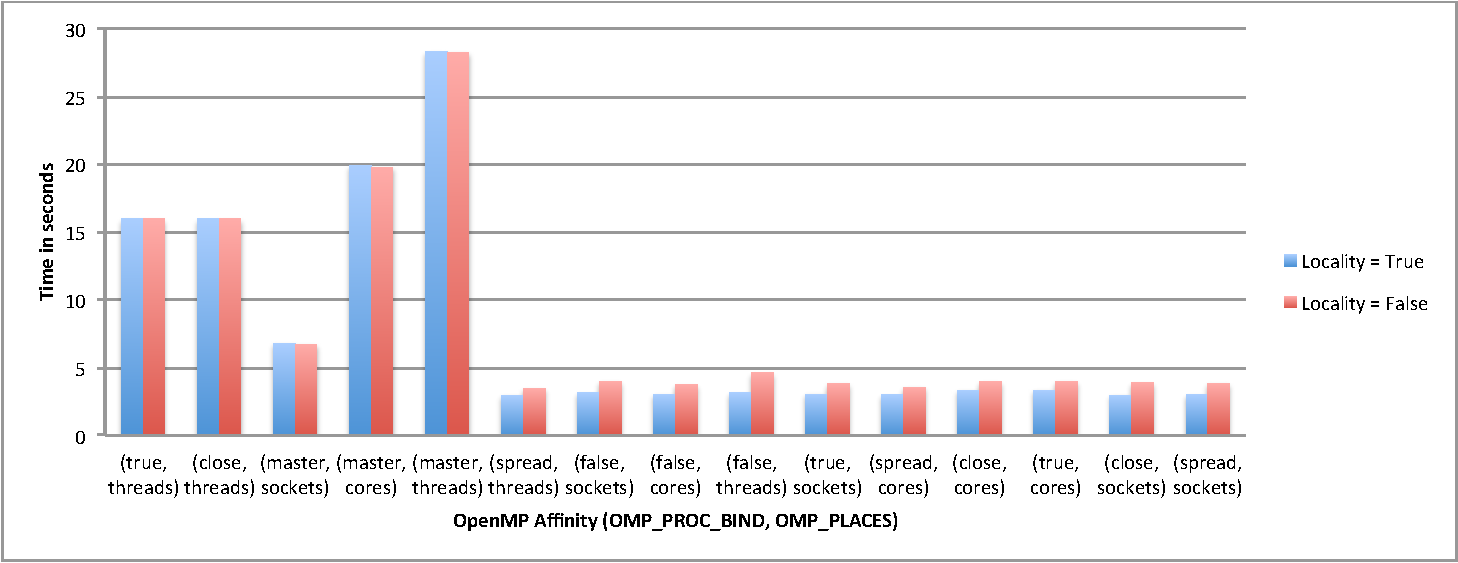
\includegraphics[height=0.4\textwidth, width=0.8\textwidth]{./Images/10Perf.pdf}
%       \caption{Performance with 10 OpenMP threads on \textit{Crest}}
%       \label{fig:10th}
%\end{figure}
%
 We experiment with the locality aware and locality unaware versions of the Jacobi program along with the default first-touch policy to observe the behavior over varying number of threads. 
 For each thread count we record the POWER8 hardware counters and the placement of the threads on the hardware. 
 Figure~\ref{fig:20th} shows the performance of 20 OpenMP threads with different OpenMP Affinity settings. We observed similar results for 10, 40, 80 and 160 OpenMP threads and hence do not show them here.
%
\begin{figure}[h!]
  \centering
  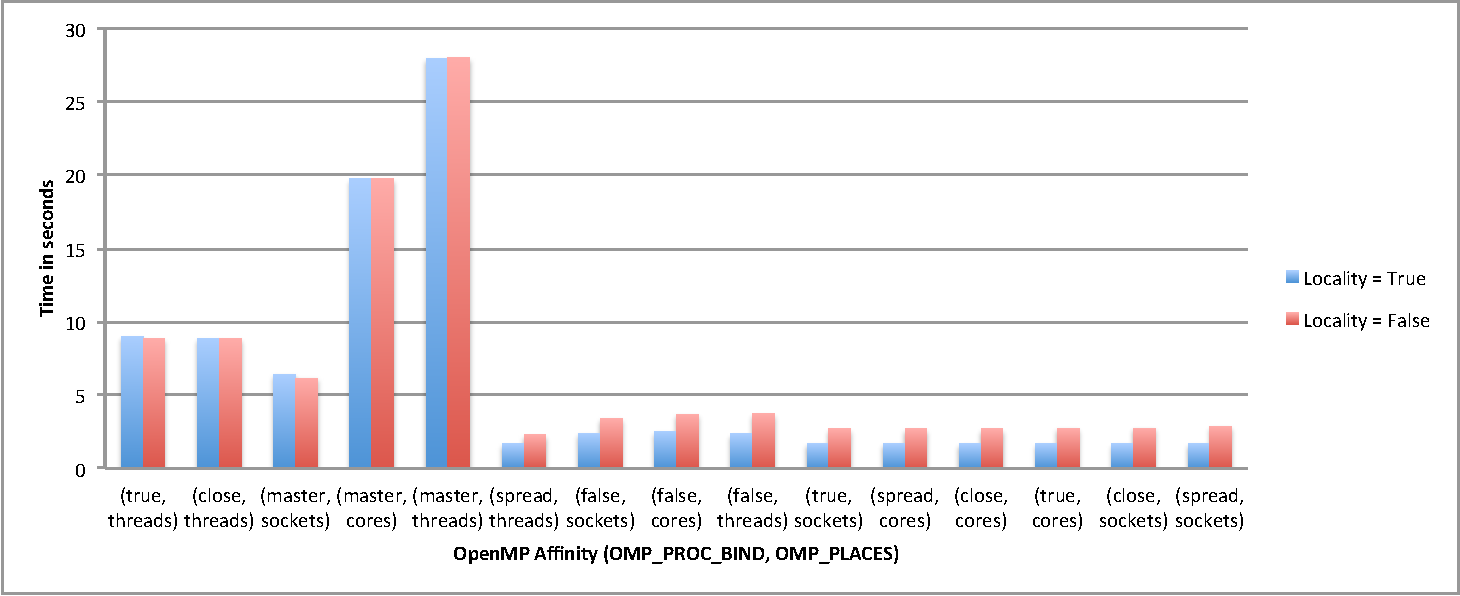
\includegraphics[height=0.4\textwidth, width=0.8\textwidth]{./Images/20Perf.pdf}
       \caption{Performance with 20 OpenMP threads on \textit{Crest}}
       \label{fig:20th}
\end{figure}
%
\begin{figure}[h!]
  \centering
  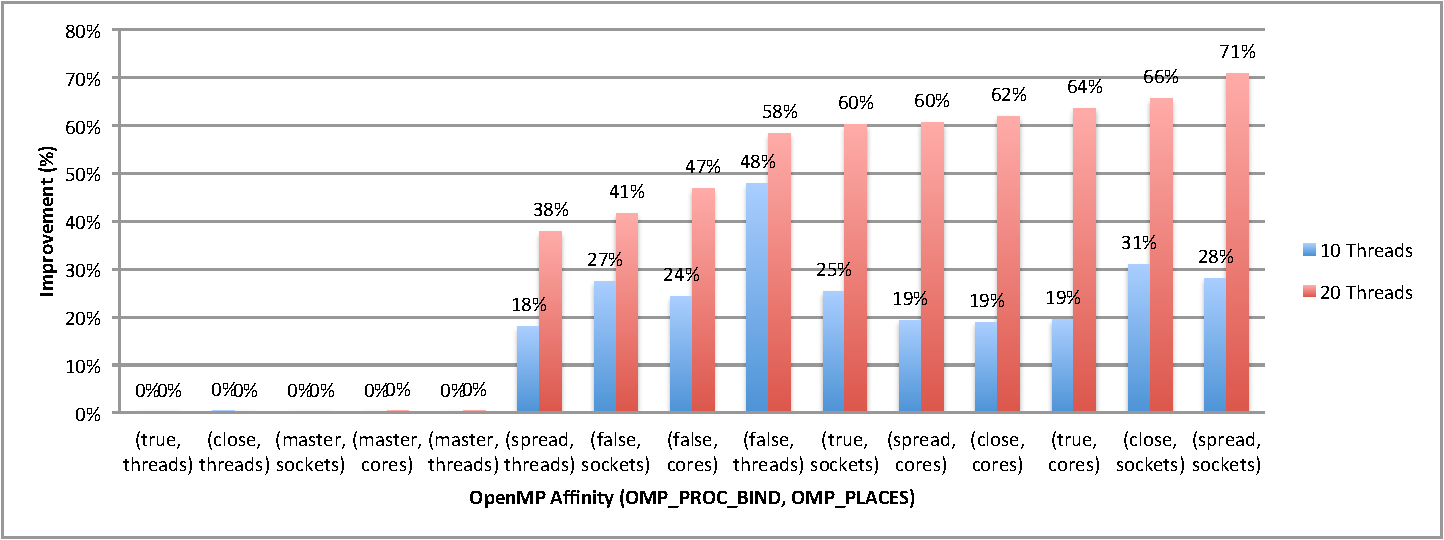
\includegraphics[height=0.4\textwidth, width=0.8\textwidth]{./Images/PerfI.pdf}
       \caption{Comparing Performance Improvement between different number of OpenMP threads}
       \label{fig:imp}
\end{figure}

For the \textit{(master, threads)} configuration all threads execute on CPUID 0. 
All threads execute in the same core as the master when the configuration is set to \textit{(master, core)}, similarly for \textit{(master, socket)} all threads execute in the same socket. In this case all threads are executing on CPUs 0 through 79 which corresponds to a single NUMA domain. When OMP\_PROC\_BIND set to master we see in Figure ~ref{fig:Imp} that there is no improvement of locality aware algorithms over non-locality aware algorithms (both using the first-touch policy).
For \textit{(close, threads)}, we observe that all OpenMP threads execute on random CPUs between 0-19. All of these cases don't suffer from memory locality issues because they access memory local to the memory within the chip.
In the \textit{(spread, sockets)} and \textit{(close, sockets)} configuration threads are spread across sockets but may be mapped to the same core. We observed that the \textit{(true, threads)} configuration is equivalent to the \textit{(close,threads)} according to the thread mappings.
For all OpenMP affinity settings  with OMP\_PROC\_BIND set to false, threads can migrate and are not bound to a specific thread, core or socket. This migration makes it less impactful on the data placement, but suffers from degraded performance.
\begin{figure}[h!]
  \centering
  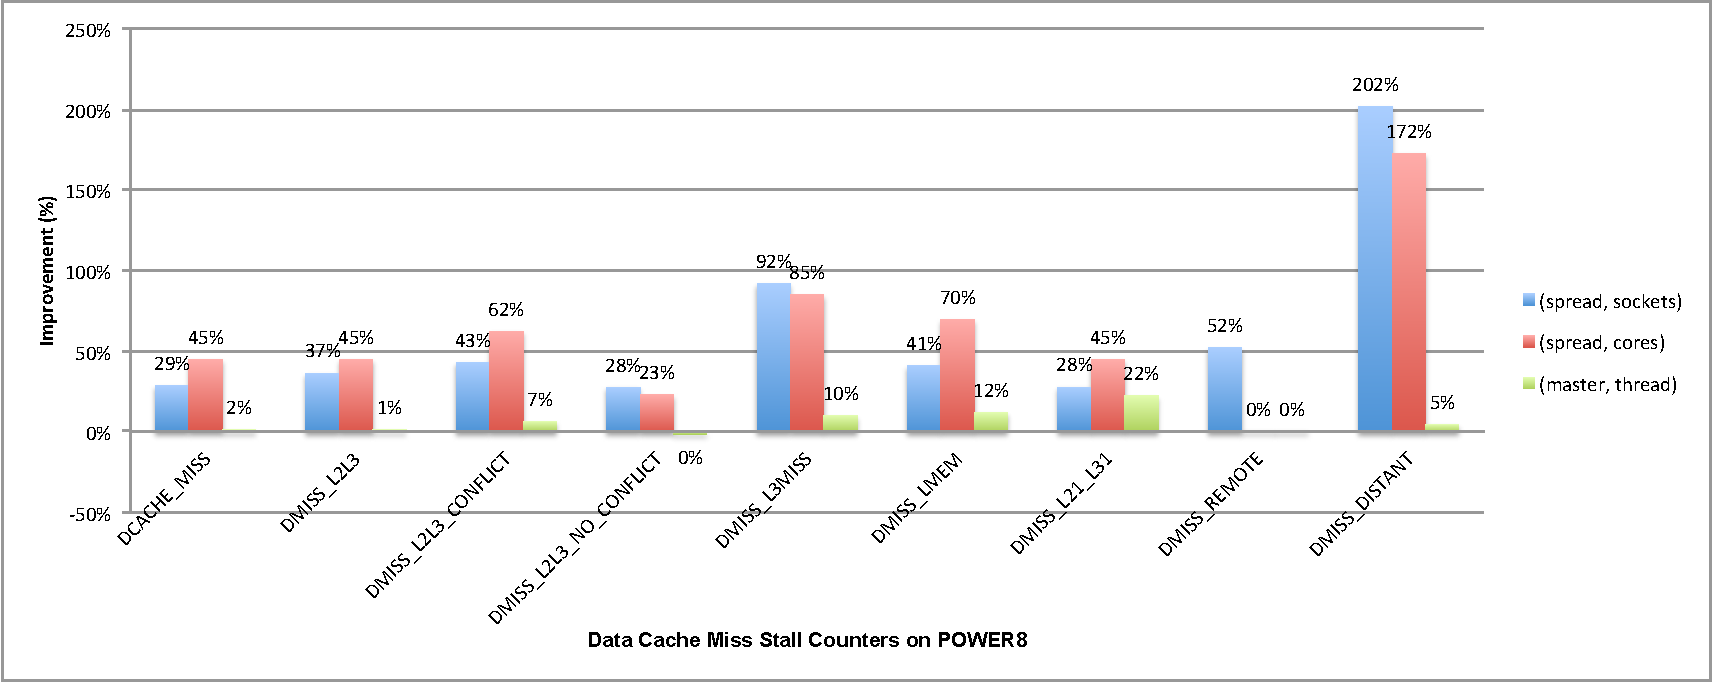
\includegraphics[height=0.4\textwidth, width=0.8\textwidth]{./Images/HW.pdf}
       \caption{Comparing Hardware Counter Change}
       \label{fig:HW}
\end{figure}
%
%Hardware Counter notes
Next we look at the hardware counters on the POWER8 system corresponding to the different configurations. 
We select the three cases of OpenMP Affinity tuple that represent the best, mid and worst improvement as seen in Figure~\ref{fig:Imp}. 
%the cases where we see more improvement for data locality on a given affinity setting 
Selected cases are \textit{(spread, sockets)},  \textit(spread, cores)}, and  \textit(master, thread)}. For these cases we record the hardware counters for the locality aware and locality unaware versions and calculate the improvement as the value of their difference as a percentage of the value of the locality unaware hardware counter value. 
From Figure~\ref{fig:HW} we see that the two hardware counters that show the effects of data locality the most are DMISS\_DISTANT, DMISS\_L3MISS.
We would have expected to see more significant variation in the value of DMISS\_REMOTE, but we found that in some cases, these remote accesses can be cached.
For example, the case of \textit{(spread, sockets)} has better DMISS\_REMOTE improvement than  \textit{(spread, cores)}. 
In (spread, sockets) some threads (not all) are running on the same core sharing local cache lines for (L1, L2) and thus taking advantage of cache reuse for remote data access. 
This can also be seen by the significant improvement in DMISS\_DISTANT which quantifies the stalls by L1 reloads from distant interventions and memory. 
The improvements we see in  \textit{(spread, cores)} are more due to DMISS\_L21\_L31, which shows a better utilization of the L2/L3 cache as this hardware counter measures the stall cycles by Dcache miss which are resolved on chip. 
In the case of  \textit{(spread, cores)} we are effectively increasing the amount of 
L2 cache available to each OpenMP thread, as each thread has access to its own L2 cache on a given core. 
For the \textit{(master, thread)} case, there is very little improvement in the memory subsystem utilization as everything is running on the same thread and the most of the data is local to the socket. In this case the data-locality version does not make any difference. This is also true for the case  \textit{(close, threads)} where
 we don't see improvements on the data locality version since data is local to the threads.


 

\section{Related Work}
\label{sec:related}
%Thread placement and migration
Thread placement can be judiciously managed by runtime systems by monitoring hardware counters and maximizing total local memory accesses across all threads for an OpenMP region~\cite{Su:2011} by factoring in the critical path. Other strategies include examining the communication patterns to discover different thread placement strategies, so that they may benefit from shared caches, through either brute force or heuristic methods~\cite{5581451}. 

%Data placement, migration, and replication
Solaris, Windows and Linux use the first-touch policy by default. To address applications that are not suited for the first-touch policy, that is, where the access patterns are not the same throughout the life of the threads~\cite{Terboven:2008} developed the next-touch policy where the data is marked to be moved to the vicinity (core or node) of the next thread accessing the data. Unfortunately this policy comes with its own set of performance issues and has not been widely accepted for scalability reasons even with improvements~\cite{Goglin:2009} such as kernel based next-touch strategy which migrates only selected pages. For many systems, it may be prudent to replicate data, instead of migrating it. This was demonstrated in~\cite{Bull02} where the cost of replication was less than migration, through they conceded that some combination of replication and migration can achieve comparable performance. Studies in~\cite{Norden:2008} focus on geographical locality for applications with dynamic access patterns and shows that migration can lead to better performance and the need for directive level migration-on-next-touch support for OpenMP applications. Data mapping suggestions and page placement for different architectures has been explored in~\cite{Smeds2003,Marathe:2006}. Up to 20\% improvement in the benchmarks��s performance was observed~\cite{Marathe:2006} when page placement was directed via feedback about the memory accesses and dynamic memory allocation. Though this study is specific to Itanium-2 general principles are applicable to all ccNUMA systems.

Dynamic thread distribution as studied by~\cite{Matthias:2009} allows multi-level thread scheduler combined with a NUMA-aware memory manager to provide hints by the runtime to be able to either re-distribute threads or migrate data upon next-touch. For providing better ccNUMA locality of data, dynamic distribution of tasks through locality aware queuing software has shown promise~\cite{DBLP:journals2011}.


\section{Conclusions and Future Work}
\label{sec:conclusion}
In this paper we evaluated OpenMP affinity support as well as memory placement on the POWER8 architecture. 
Data locality and affinity are key concepts to exploit the compute and memory capabilities to achieve good performance by minimizing data motion across NUMA domains. 
The main contribution of this paper is to evaluate current affinity features of OpenMP 4.0 on the POWER8 processors, and on how to measure its effects on data locality on a system with two P8 sockets. 
%What we observe from the experiments is that the effect of data placement and data locality is dependent on how threads are mapped to the architectures. 
In some OpenMP affinity test cases, we show that the POWER8 architecture, using its NUCA L3 caches, can hide the cost of accessing remote memory (e.g, as shown in the experiment \textit{(spread, cores)} when running a thread per core since maximizes local caches are available per thread. 
In other cases, when threads share some of the cores, there is a benefit of cache reuse in the non-shared L2 and L1 caches thus improving data locality in the application.
 In this paper we show that optimizing an application for data locality, the improvements will depend on the kind of affinity used. 

Future version of OpenMP affinity model need to support better the concept of NUMA domains. 
This is possibly another \textit{place} option called \textit{Numa} can be added to OpenMP 5.0 via the \emph{OMP\_PLACES} so that threads can be mapped more efficiently to NUMA domains. Although this can be achieved by using OS supported bindings (\textit{taskset} on linux platforms), it is not a portable mechanism. By introducing the support of NUMA domains at the OpenMP level, we can keep the implementation details opaque from the programmer while providing a portable solution across all architectures.


Another type of extensions is to integrate the concept of OMP\_PLACES with the OpenMP target directive and device\_num. Our next step would be to explore ways of mapping OpenMP \emph{target} and \emph{target data} 
regions to NUMA domains to control data and thread placement.



% conference papers do not normally have an appendix

%\section{Acknowledgments}
%This research used resources of the Oak Ridge Leadership Computing Facility at the Oak Ridge National Laboratory, 
which is supported by the Office of Science of the U.S. Department of Energy under Contract No. DE-AC05-00OR22725.


\bibliographystyle{splncs}
\bibliography{references}

\end{document}
